\section{Design}
\label{sec:design}

\subsection{Secure Isolation}
The two primary goals of our design is to a. Provide isolation of selected applications on mobile phones and b. To build a usable solution which can be integrated seamlessly into the host operating system of the smartphone. To achieve these goals we either need a type-II hypervisor which can run within the host operating system or employ OS-level virtualization techniques like containers.  Unlike conventional virtualization, containers have almost no overhead as they do not run the entire software stack of the guest operating system.  On the other hand, because the virtualization is facilitated by the operating system, other OSes or architectures cannot be used within a container.  In our design, we propose to use operating system level virtualization techniques of which Linux Containers and OpenVZ \cite{OpenVZ} are popular implementations.\\
 
\subsection{Linux Containers}
Linux Containers (LXC) implement OS-level virtualization techniques in order to run a number of isolated virtual environments on a single host.  LXC differs from conventional virtualization techniques, which generally require the installation of guest OSes.  The isolated virtual environments or containers, are built upon other Linux security mechanisms \cite{LSM}. We list the different resources isolated using containers and the techniques used for them below.

\begin{figure}[tbh]
\centering
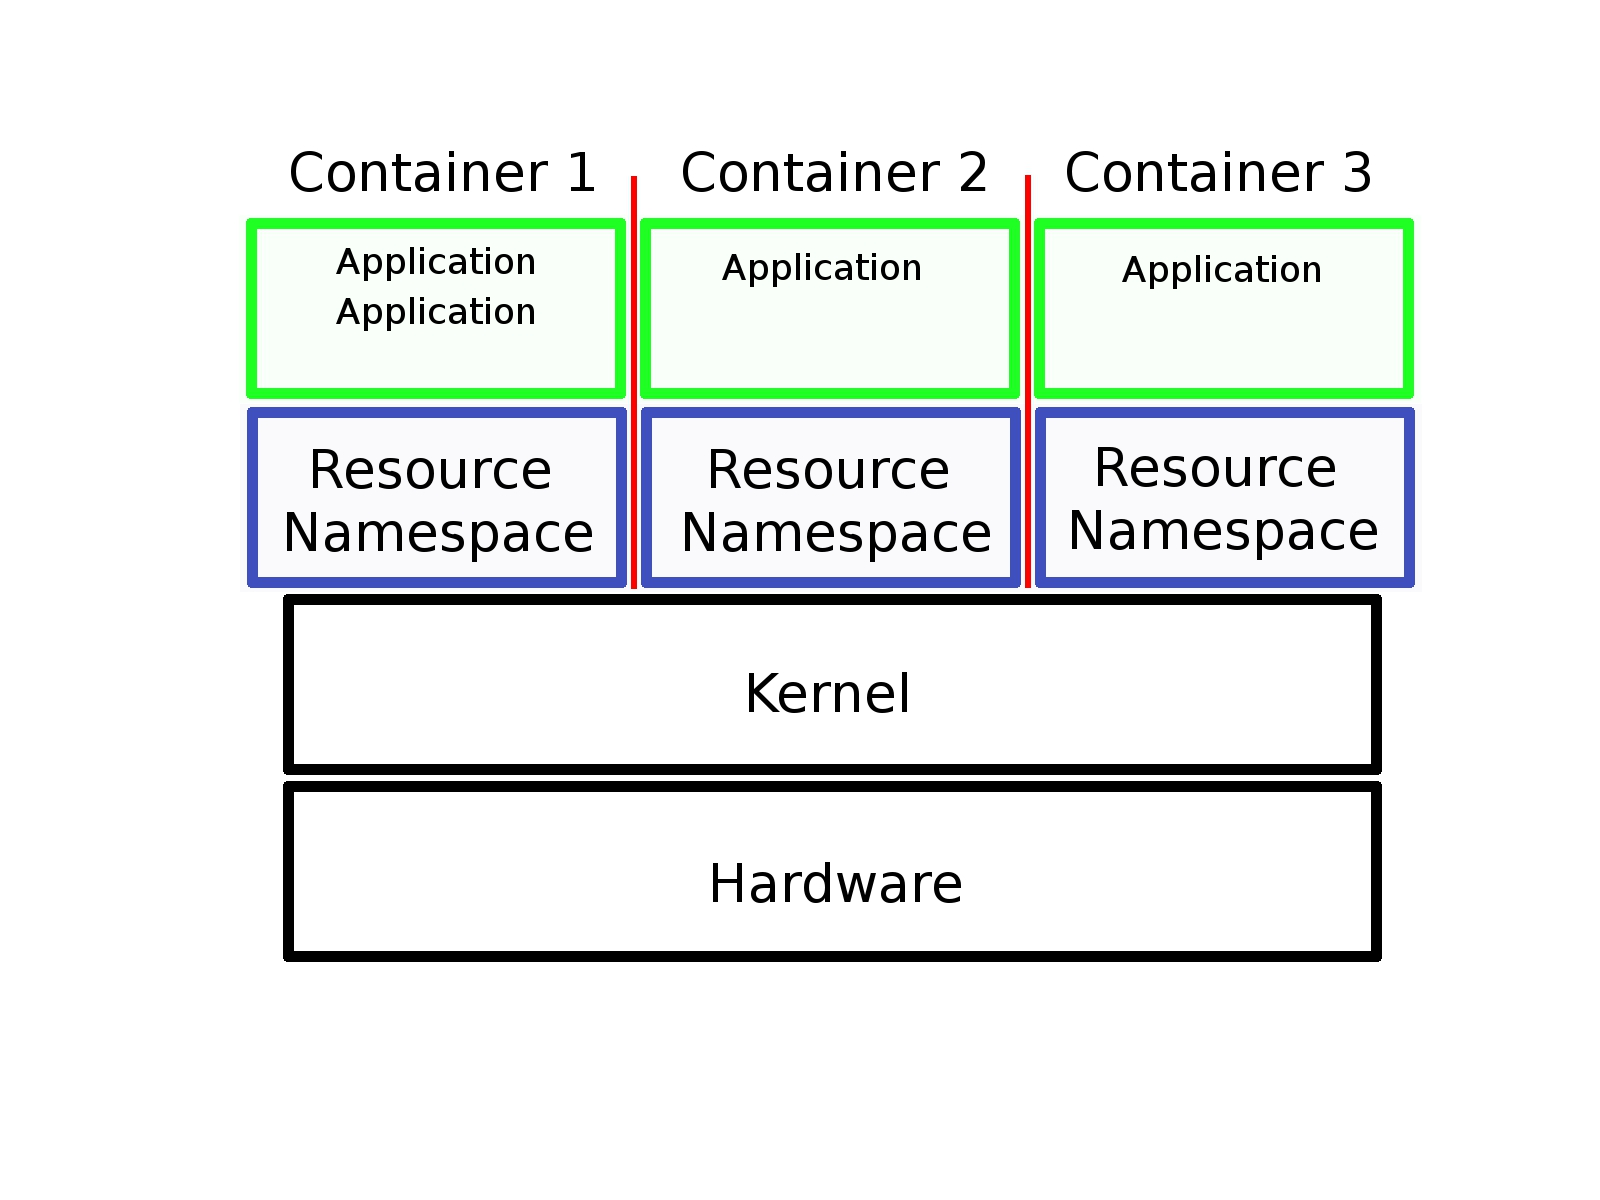
\includegraphics[width=1.0\columnwidth]{containers}
\caption{Linux Container Architecture}
\label{fig:containers}
\end{figure}


\subsection{Host Identification}
On Linux machines, the identity of a system is usually established through the command `uname'. This command reads information stored in the structure `utsname'. The structure includes the name of the operating system in use and the current version of the operating system. The structure also contains the hostname of the machine and this is used to identify the machine in network communications. Linux Containers implement a per-process utsname namespace and this enables each container to have a different hostname.

\subsection{Process Identifiers}
Process identifiers (PIDs) are isolated using PID namespaces such that with respect to each container the set of PIDs appears like a standalone machine. This also allows two processes to  have the same PID in different containers. Processes can be launched in a new PID namespace using the clone or the unshare system-calls. This is an important feature for enabling migration of containers between hosts as the same PID values can be maintained at the source and destination. Also, PID namespaces are hierarchical; tasks in the original namespace can see the PIDs of tasks in the new namespace but not vice-versa.  

\subsection{Inter-Process Communications}
Inter-Process Communication (IPC) between processes uses shared objects like shared memory segments, message queues etc. To create isolated environments, it is necessary that processes from one container cannot share data or communicate with other containers. This is achieved by introducing IPC namespaces which creates separate set of IPC objects for each container.

\subsection{User Namespaces}
User namespaces were first available in Linux kernel 2.6.23.  User namespaces supplies additional uid tables in order to allow a uid to be namespace specific.  With user namespaces, different users can be associated with the same uid across different processes.

\subsection{Network Devices}
The Linux kernel version 2.6.26 was the first version to include namespaces for network devices.  The network namespaces assign a private set of network resources, including IP addresses, routes, sockets to any number of processes.  This allows for shared names among different namespaces and isolation between those namespaces.  This provides substantial improvements in security, network resource management, namespace consolidation, and mobility. Network namespaces are implemented using virtual ethernet devices and containers can bind to the same ports without interfering with each other. This is a useful feature as, for example, we could have two webservers listen on port $80$ in different containers.

%% Leaving out
%% \subsection{\\Proc Namespaces}

\subsection{Readonly-bind mounts}
Readonly-bind mounts have been available since Linux kernel 2.6.24.  This allows for read-only accesses to a filesystem mounted read-write.  It guarantees that one process can read and write to the filesystem, while others can only read from it, regardless of their privileges.

\subsubsection{Copy-on-Write filesystems}
One of the techniques used to prevent duplication of system directories such as /bin, /lib across containers is to mount them as read-only bind mounts from native system into a container. However this means that processes running within containers would be restricted and not able to perform tasks like installing new binaries into /bin. In order to enable each container to make modifications to the system directories and avoid making multiple copies, we use Unionfs \cite{tos06unionfs} a file-level copy-on-write filesystem. 

Unionfs is a file system which aims to maintain UNIX semantics while providing advanced namespace-unification capabilities. It allows read-only and read-write branches to be inserted into the same tree, handles elimination of duplicates and provides support for snapshots. Unionfs is often used in scenarios where a base OS image is provided on a read-only CD-ROM and any changes made the user are stored in a separate read-write directory. Our use-case is similar as the phone's native OS image is mounted read-only and any changes made by each container is stored in its own separate read-writeable directory.

\subsection{Other features}
In addition to the above mentioned isolation features, the Linux Container project adds support for \emph{Control Groups} which can be used to limit the resources used by a container. Additionally, capability bounds can be used to restrict the privileges of a container and these features help ensure that the resources in a machine can be isolated and fairly shared between different containers.
